%% (Master) Thesis template
% Template version used: v2
%
% Largely adapted from Adrian Nievergelt's template for the ADPS
% (lecture notes) project.

%% We use the memoir class because it offers many easy to use features.
% Template v2 fixes:
% Removed titlepage from options: LaTeX Warning: Unused global option(s): [titlepage].
% Electronic version that does not waste space
\documentclass[11pt,a4paper,openany,oneside]{memoir}
% Printable version that does waste space (but people like it), uncomment for printing
% \documentclass[11pt,a4paper]{memoir}

%% Packages
%% ========

%% LaTeX Font encoding -- DO NOT CHANGE
\usepackage[OT1]{fontenc}

%% Babel provides support for languages.  'english' uses British
%% English hyphenation and text snippets like "Figure" and
%% "Theorem". Use the option 'ngerman' if your document is in German.
%% Use 'american' for American English.  Note that if you change this,
%% the next LaTeX run may show spurious errors.  Simply run it again.
%% If they persist, remove the .aux file and try again.
\usepackage[english]{babel}

%% Input encoding 'utf8'. In some cases you might need 'utf8x' for
%% extra symbols. Not all editors, especially on Windows, are UTF-8
%% capable, so you may want to use 'latin1' instead.
\usepackage[utf8]{inputenc}

%% This changes default fonts for both text and math mode to use Herman Zapfs
%% excellent Palatino font.  Do not change this.
\usepackage[sc]{mathpazo}

%% The AMS-LaTeX extensions for mathematical typesetting.  Do not
%% remove.
\usepackage{amsmath,amssymb,amsfonts,mathrsfs}

%% NTheorem is a reimplementation of the AMS Theorem package. This
%% will allow us to typeset theorems like examples, proofs and
%% similar.  Do not remove.
%% NOTE: Must be loaded AFTER amsmath, or the \qed placement will
%% break
\usepackage[amsmath,thmmarks]{ntheorem}

%% LaTeX' own graphics handling
\usepackage{graphicx}

%% We unfortunately need this for the Rules chapter.  Remove it
%% afterwards; or at least NEVER use its underlining features.
\usepackage{soul}

%% This allows you to add .pdf files. It is used to add the
%% declaration of originality.
\usepackage{pdfpages}

%% Some more packages that you may want to use.  Have a look at the
%% file, and consult the package docs for each.
%% See the TeXed file for more explanations

%% [OPT] Multi-rowed cells in tabulars
%\usepackage{multirow}

%% Make document internal hyperlinks wherever possible. (TOC, references)
%% This MUST be loaded before cleveref
\usepackage[linkcolor=black,colorlinks=true,citecolor=black,filecolor=black]{hyperref}

%% [REC] Intelligent cross reference package. This allows for nice
%% combined references that include the reference and a hint to where
%% to look for it.
%% Template v2: cleveref already recognizes what is being referenced - one does not need to write Fig./Sec.
% \usepackage{varioref}. Capitalization is prefered in CS
\usepackage[capitalise]{cleveref}

%% [OPT] Easily changeable quotes with \enquote{Text}
\usepackage[german=swiss]{csquotes}

%% Template v2: this prevents warning "Package fmtcount Warning: \ordinal already defined use \FCordinal instead. on input line". See https://tex.stackexchange.com/questions/162353/memoir-class-conflict-with-datetime#comment371926_162358
\let\ordinal\relax
%% [REC] Format dates and time depending on locale
\usepackage{datetime}

%% [OPT] Provides a \cancel{} command to stroke through mathematics.
%\usepackage{cancel}

%% [NEED] This allows for additional typesetting tools in mathmode.
%% See its excellent documentation.
\usepackage{mathtools}

%% [ADV] Conditional commands
%\usepackage{ifthen}

%% [OPT] Manual large braces or other delimiters.
%\usepackage{bigdelim, bigstrut}

%% [REC] Alternate vector arrows. Use the command \vv{} to get scaled
%% vector arrows.
\usepackage[h]{esvect}

%% [NEED] Some extensions to tabulars and array environments.
\usepackage{array}

%% [OPT] Postscript support via pstricks graphics package. Very
%% diverse applications.
%\usepackage{pstricks,pst-all}

%% [?] This seems to allow us to define some additional counters.
%\usepackage{etex}

%% [ADV] XY-Pic to typeset some matrix-style graphics
%\usepackage[all]{xy}

%% [OPT] This is needed to generate an index at the end of the
%% document.
%\usepackage{makeidx}

%% [OPT] Fancy package for source code listings.  The template text
%% needs it for some LaTeX snippets; remove/adapt the \lstset when you
%% remove the template content.
\usepackage{listings}
\lstset{language=TeX,basicstyle={\normalfont\ttfamily}}

% Template v2 fixes: this is an old package, microtype is superior + fixes an error
%% [REC] Fancy character protrusion.  Must be loaded after all fonts.
\usepackage[activate]{microtype}
% \usepackage[activate]{pdfcprot}  % causes the compilation error

%% [REC] Nicer tables.  Read the excellent documentation.
\usepackage{booktabs}


%% Our layout configuration.  DO NOT CHANGE.
%% Memoir layout setup

%% NOTE: You are strongly advised not to change any of them unless you
%% know what you are doing.  These settings strongly interact in the
%% final look of the document.

% Dependencies
\usepackage{eth-template/ETHlogo}

% Turn extra space before chapter headings off.
\setlength{\beforechapskip}{0pt}

\nonzeroparskip
\parindent=0pt
\defaultlists

% Chapter style redefinition
\makeatletter

\if@twoside
  \pagestyle{Ruled}
  \copypagestyle{chapter}{Ruled}
\else
  \pagestyle{ruled}
  \copypagestyle{chapter}{ruled}
\fi
\makeoddhead{chapter}{}{}{}
\makeevenhead{chapter}{}{}{}
\makeheadrule{chapter}{\textwidth}{0pt}
\copypagestyle{abstract}{empty}

\makechapterstyle{bianchimod}{%
  \chapterstyle{default}
  \renewcommand*{\chapnamefont}{\normalfont\Large\sffamily}
  \renewcommand*{\chapnumfont}{\normalfont\Large\sffamily}
  \renewcommand*{\printchaptername}{%
    \chapnamefont\centering\@chapapp}
  \renewcommand*{\printchapternum}{\chapnumfont {\thechapter}}
  \renewcommand*{\chaptitlefont}{\normalfont\huge\sffamily}
  \renewcommand*{\printchaptertitle}[1]{%
    \hrule\vskip\onelineskip \centering \chaptitlefont\textbf{\vphantom{gyM}##1}\par}
  \renewcommand*{\afterchaptertitle}{\vskip\onelineskip \hrule\vskip
    \afterchapskip}
  \renewcommand*{\printchapternonum}{%
    \vphantom{\chapnumfont {9}}\afterchapternum}}

% Use the newly defined style
\chapterstyle{bianchimod}

\setsecheadstyle{\Large\bfseries\sffamily}
\setsubsecheadstyle{\large\bfseries\sffamily}
\setsubsubsecheadstyle{\bfseries\sffamily}
\setparaheadstyle{\normalsize\bfseries\sffamily}
\setsubparaheadstyle{\normalsize\itshape\sffamily}
\setsubparaindent{0pt}

% Set captions to a more separated style for clearness
\captionnamefont{\sffamily\bfseries\footnotesize}
\captiontitlefont{\sffamily\footnotesize}
\setlength{\intextsep}{16pt}
\setlength{\belowcaptionskip}{1pt}

% Set section and TOC numbering depth to subsection
\setsecnumdepth{subsection}
\settocdepth{subsection}

%% Titlepage adjustments
\pretitle{\vspace{0pt plus 0.7fill}\begin{center}\HUGE\sffamily\bfseries}
\posttitle{\end{center}\par}
\preauthor{\par\begin{center}\let\and\\\Large\sffamily}
\postauthor{\end{center}}
\predate{\par\begin{center}\Large\sffamily}
\postdate{\end{center}}

\def\@advisors{}
\newcommand{\advisors}[1]{\def\@advisors{#1}}
\def\@department{}
\newcommand{\department}[1]{\def\@department{#1}}
\def\@thesistype{}
\newcommand{\thesistype}[1]{\def\@thesistype{#1}}

\renewcommand{\maketitlehooka}{\noindent\ETHlogo[2in]}

\renewcommand{\maketitlehookb}{\vspace{1in}%
  \par\begin{center}\Large\sffamily\@thesistype\end{center}}

\renewcommand{\maketitlehookd}{%
  \vfill\par
  \begin{flushright}
    \sffamily
    \@advisors\par
    \@department, ETH Z\"urich
  \end{flushright}
}

\checkandfixthelayout

\setlength{\droptitle}{-48pt}

\makeatother

% This defines how theorems should look. Best leave as is.
\theoremstyle{plain}
\setlength\theorempostskipamount{0pt}

% These lines adjust the left and right margins
\setlrmarginsandblock{3.3cm}{3.3cm}{*}
\checkandfixthelayout

%%% Local Variables:
%%% mode: latex
%%% TeX-master: "thesis"
%%% End:


%% Theorem environments.  You will have to adapt this for a German
%% thesis.
%% Theorem-like environments

%% This can be changed according to language. You can comment out the ones you
%% don't need.

\numberwithin{equation}{chapter}

%% German theorems
%\newtheorem{satz}{Satz}[chapter]
%\newtheorem{beispiel}[satz]{Beispiel}
%\newtheorem{bemerkung}[satz]{Bemerkung}
%\newtheorem{korrolar}[satz]{Korrolar}
%\newtheorem{definition}[satz]{Definition}
%\newtheorem{lemma}[satz]{Lemma}
%\newtheorem{proposition}[satz]{Proposition}

%% English variants
\newtheorem{theorem}{Theorem}[chapter]
\newtheorem{example}[theorem]{Example}
\newtheorem{remark}[theorem]{Remark}
\newtheorem{corollary}[theorem]{Corollary}
\newtheorem{definition}[theorem]{Definition}
\newtheorem{lemma}[theorem]{Lemma}
\newtheorem{proposition}[theorem]{Proposition}

%% Proof environment with a small square as a "qed" symbol
\theoremstyle{nonumberplain}
\theorembodyfont{\normalfont}
\theoremsymbol{\ensuremath{\square}}
\newtheorem{proof}{Proof}
%\newtheorem{beweis}{Beweis}


%% Helpful macros.
%% Custom commands
%% ===============

%% Special characters for number sets, e.g. real or complex numbers.
\newcommand{\C}{\mathbb{C}}
\newcommand{\K}{\mathbb{K}}
\newcommand{\N}{\mathbb{N}}
\newcommand{\Q}{\mathbb{Q}}
\newcommand{\R}{\mathbb{R}}
\newcommand{\Z}{\mathbb{Z}}
\newcommand{\X}{\mathbb{X}}

%% Fixed/scaling delimiter examples (see mathtools documentation)
\DeclarePairedDelimiter\abs{\lvert}{\rvert}
\DeclarePairedDelimiter\norm{\lVert}{\rVert}

%% Use the alternative epsilon per default and define the old one as \oldepsilon
\let\oldepsilon\epsilon
\renewcommand{\epsilon}{\ensuremath\varepsilon}

%% Also set the alternate phi as default.
\let\oldphi\phi
\renewcommand{\phi}{\ensuremath{\varphi}}


% Template v2: BibLaTeX with Biber backend are in my opinion best maintainable citation configurations. IEEE style is common in CS.
% Bibliography
\usepackage[
bibstyle=ieee,
citestyle=numeric,
isbn=true,
doi=true,
sorting=none,
url=true,
% defernumbers=true,
bibencoding=utf8,
backend=biber
]{biblatex} %Imports BibLaTeX package
\addbibresource{refs.bib} %Import the bibliography file

%% Document information
%% ====================

\title{Relating compound toxicity to molecular structure using machine learning}
\author{Robin Bosshard}
\thesistype{Master Thesis}
\advisors{Advisors: Dr.\ Eliza Harris, Dr.\ K. Arturi, Lilian Gasser}
\department{Department of Computer Science}
\date{October 16, 2023}

\begin{document}

\frontmatter

%% Title page is autogenerated from document information above.  DO
%% NOT CHANGE.
\begin{titlingpage}
  \calccentering{\unitlength}
  \begin{adjustwidth*}{\unitlength-24pt}{-\unitlength-24pt}
    \maketitle
  \end{adjustwidth*}
\end{titlingpage}

%% The abstract of your thesis.  Edit the file as needed.
\begin{abstract}
  This thesis enhances the MLinvitroTox framework, which predicts the toxicity of unknown compounds from High-Resolution Mass-Spectrometry (HRMS/MS) fragmentation spectra data. This framework forecasts the most hazardous compounds in environmental samples, circumventing the need for resource-intensive chemical identification. The predictivity is evaluated on SIRIUS molecular fingerprints from MassBank spectra data. However, the machine learning models are trained on molecular fingerprints from structure and uses in vitro toxicity data from ToxCast/Tox21. We have developed pytcpl, a Python-based processing pipeline that extends its applicability to the latest toxicity data. We have employed datasets for various assay endpoints, encompassing diverse aspects of toxicity. The individual machine learning models achieve an average balanced accuracy of todo:X when predicting binary toxicity, and they also demonstrate effectiveness when validated using MassBank spectra data. Furthermore, we've created a user-friendly web app to facilitate interaction with this framework.
\end{abstract}


%% TOC with the proper setup, do not change.
\cleartorecto
\tableofcontents
\mainmatter

%% Your real content!
% Some commands used in this file
\newcommand{\package}{\emph}

\chapter{Introduction}\label{chap:introduction}

\section{The Challenge of Environmental Pollution}

Over the past few decades, the upsurge in environmental pollution by chemical compounds has been driven by industrial processes, agricultural methods, our consumerism and various other contributing factors. This has resulted in significant ecological and health issues. Although these chemicals are integral for many products and have the potential to improve our comfort of modern society, they can also pose risks and adversely affect both our health and the environment, either acutely or chronically. Toxic substances threaten wildlife but also makes our air, soil and finally our drinking water and food supply less safe. The EU currently maintains comprehensive chemical regulations, however, it is anticipated that global chemicals production will double by 2030~\cite{chemicaloutlook}. Moreover, the widespread utilization of chemicals, including their inclusion in consumer goods, is expected to expand further.
Even though there are over 275 million known chemical compounds registered by the Chemical Abstracts Service (CAS)~\cite{CAS}, merely a tiny fraction of them undergo close monitoring via target analytical approaches and even less is known about their toxicity profiles and negative health effects on our organsims.

Building upon the European Green Deal~\cite{greendeal}, the 8th Environment Action Programme, guiding European environmental policy until 2030, reinforces the EU's goal of sustainable living within planetary limits, with a vision extending to 2050. One of its key objectives is a zero-pollution commitment, covering air, water, and soil, prioritizing the well-being of EU citizens. In particular, the European Commission published a sustainability-focused chemicals strategy (CSS), aligning with the EU's zero-pollution ambition with one of the objectives to minimize concerning substances by either substituting or phasing them out wherever feasible~\cite{EUChemicalsStrategy}. 
Consequently, the urgent need to monitor and effectively assess the hazards associated with the daily entering of thousands of poorly understood chemicals into our environment becomes increasingly evident.

\section{The Imperative for Prioritization and Toxicity Assessment}

Modern analytical methods, especially high-resolution mass spectrometry (HRMS/MS), are becoming increasingly important in fields like metabolomics, drug discover, forensics and environmental science and toxicology. Nontarget HRMS/MS has improved the ability to detect emerging compounds in environmental samples, often with unknown toxicity profiles. These compounds are assessed based on factors such as abundance and fragmentation data. See in Figure~\ref{fig:non_target_high_resolution_mass_spectrometry} for an overview. However, the endeavor to identify compounds and characterize their toxicity remains a resource-intensive and time-consuming process. This challenge is further impeded by the scarcity of well-characterized substances that can be used as references for comparison when analyzing unknown compounds, hindering comprehensive elucidation. Traditionally, the prioritization of unidentified compounds rely on signal intensity as a guiding metric. Unfortunately, this approach falls short in delivering an accurate assessment of environmental exposures, as it tends to overlook the crucial toxicological dimension. Consequently, substances with the potential for severe ecological consequences, such as endocrine-disrupting compounds, frequently evade detection due to their low abundance, despite their high toxicity. Therefore, there is an urgent need for alternative hazard-driven prioritization strategies of unidentified NTS HRMS/MS signals that incorporate the toxicity and ecological impact more effectively.

\begin{figure}[htbp]  % Placement options: h (here), t (top), b (bottom), p (page)
    \centering
    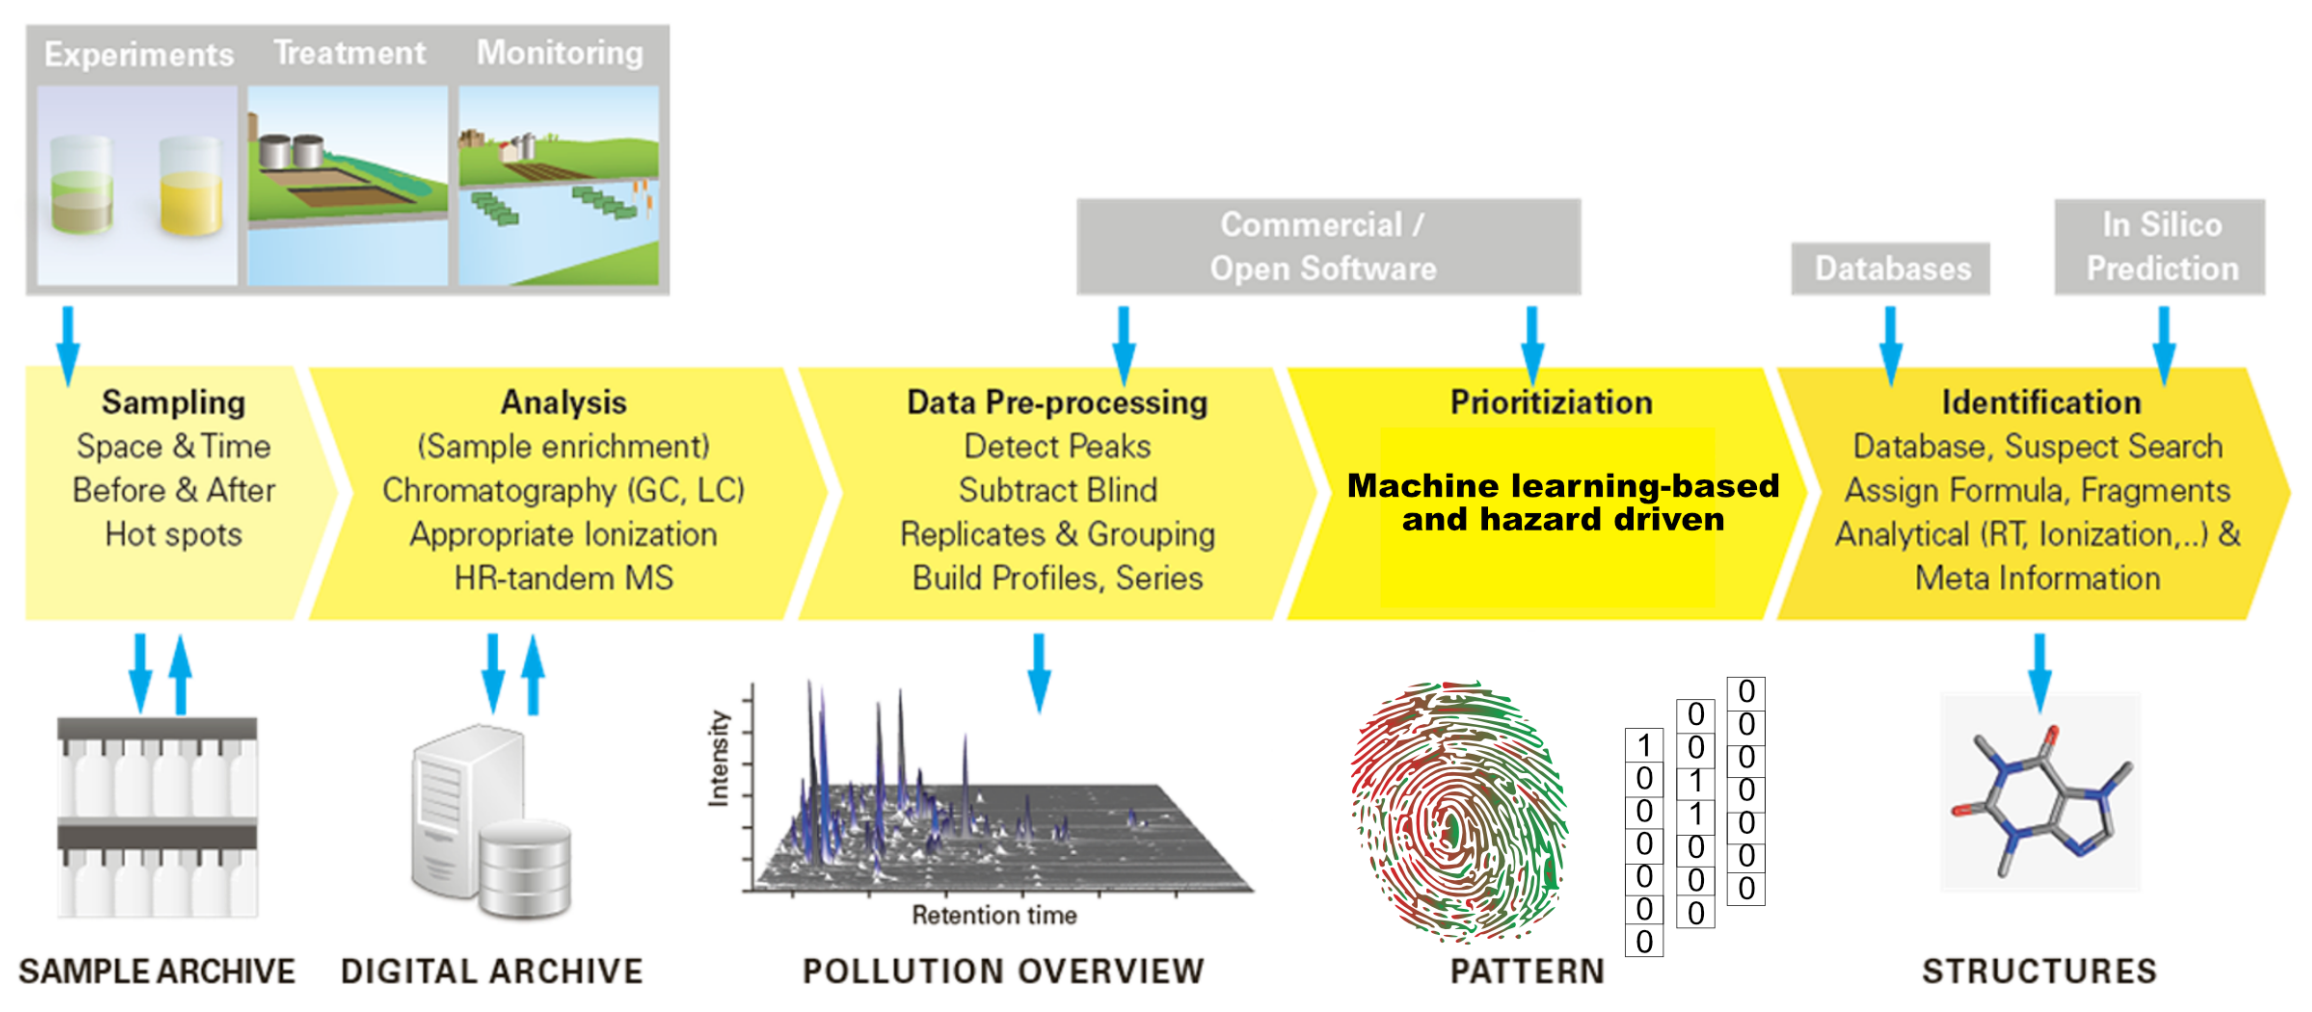
\includegraphics[width=1.0\textwidth]{figures/non_target_high_resolution_mass_spectrometry_1.png}  
    \caption{Figure 1 adapted (with modified Prioritization step) from Hollender et al.~\cite{hollender}: Nontarget screening with high resolution mass spectrometry in the environment: Ready to go? }
~\label{fig:non_target_high_resolution_mass_spectrometry} 
\end{figure}

\section{The Promise of Machine Learning in Toxicity Prediction}

In the past few years, machine learning has emerged as a transformative force in the field of toxicology, particularly in the realm of high-throughput toxicity prediction. High-throughput screening (HTS) has revolutionized the way we assess toxicity by allowing thousands of in vitro bioassays to be conducted rapidly. This high-throughput approach, coupled with advancements in robotics and automated analysis, has generated large volumes of toxicity data, paving the way for more comprehensive assessments of chemical compounds.
Alongside the rise of machine learning, this advancement has facilitated the creation of predictive models capable of forecasting compound toxicity based on their chemical structure. These models can be trained on extensive datasets containing well-documented toxicity information, allowing them to learn the underlying patterns and relationships between chemical structure and target toxicity. Once trained, these models can reliably predict the toxicity of new compounds, even if they have not undergone laboratory testing. This approach holds the potential to significantly reduce the time and cost associated with early-stage toxicity pre-assessment and plays a crucial role in prioritizing compounds for further in-depth testing.

\section{MLinvitroTox: A Novel Approach}

In response to the pressing need for a more hazard-driven and comprehensive assessment of environmental contaminants, Arturi et al. introduced MLinvitroTox~\cite{arturi}, an innovative machine learning framework. In particular it is the primary goal of this thesis to collaborate with the authors in further advancing and developing this framework. MLinvitroTox leverages molecular fingerprints extracted from fragmentation spectra~\footnote{also termed as Tandem mass spectrometry or MS/MS or MS2}, marking a fundamental shift in how we forecast the toxicity of the myriad unidentified HRMS/MS features. While traditional QSAR models predict bioactivities based on molecular fingerprints derived from chemical structures, MLinvitroTox was trained with supervised classification models on molcular fingerprints from chemical structures but is applied to molecular fingerprints generated from experimentally measured MS2 spectra using \emph{SIRIUS} and \emph{CSI:FingerID}. SIRIUS is a software package for annotating small molecules from nontarget HRMS/MS data, while CSI:FingerID is a machine-learning tool employed by SIRIUS to predict molecular fingerprints from fragmentation spectra. MLinvitroTox leverages streamlined machine learning techniques to predict the compounds bioactivity, respectively toxicity, ensuring a broad toxicological coverage encompassing nearly 300 target-specific and 90 cytotoxic endpoints, sourced from ToxCast/Tox21 data. Subsequently, the toxicity predictions generated by the framework are employed to prioritize compounds, with the flexibility to emphasize specific aspects of toxicity profiles tailored to individual preferences. This prioritization strategy facilitates more streamlined and thorough evaluations of environmental contaminants, enhancing a more hazard-driven risk assessment.


Kommentar (zentrale Frage, todo: für mich nicht ganz klar): Verständins vom Anwendugszweck von MLinvitroTox noch nicht ganz klar. Warum berechnet man nicht einmalig eine vollständige Tabelle mit allen potenziellen Chemikalien die im MS2 Spektrum auftreten könnten und predicted deren toxicity fingerprints und kann dann für neue environment samples einen simplen Lookup machen? Anstatt die toxicity profiles jedes Mal aufs Neue zu predicten mit einer pipeline und dann eine hazard-driven prioritization vornehmen? Meine Frage ist, wenn man die Rangliste von Chemikalien hat, sortiert nach Toxicity, warum kann man nicht einfach danach statisch priorisieren mit einem purem hazard-driven approach, warum braucht es dann eine dynamische pipeline?. Welche Komponente fehlt in dieser Logik damit die pipeline nötig ist? Vielleicht wenn neue Chemikalien/Daten dazu kommen. Will man das, weil der User den Fokus auf Toxicity-fingerprint anders legen will und dann basierend auf diesen Variabel, die Menge an Chemikalien für weiterführende gründliche analytische Tests anders priorisiert ist? Zum Beispiel, fokusiere auf Chemikalien, die ein hohes Risiko auf unser Hormon-System haben? Aber gleichermassen auch hier kann die Annahme gemacht werden, dass die toxicity fingerprints bekannt (predicted ahead) sind, wenn man das einmal gemacht hat für alle Chemikalien. Dann würde aus meiner Sicht ein einfaches Programm reichen für den Anweduungsfall, das nur die gewünschten Abschnitte (target) des toxicity fingerprint fokusiert und dann die Chemikalien nach target Toxicity sortiert und dies die besagte Priorisierung ist? Oder ist das zu einfach gedacht? 



\section{Objectives and Significance}

The central objective of this thesis is to develop a streamlined framework for the prediction of compound toxicity across multiple endpoints, resulting in the creation of toxicity fingerprint. The generated toxicity fingerprints will provide valuable insights for the prioritization process in identifying most hazardous compounds found in environmental samples, ultimately contributing to the preservation of ecosystems and our health. The framework aims to develop a custom curation of structural and toxicological data to address challenges from modeling heterogenuous, and imbalanced data sets. Notably, the use of SIRIUS molecular fingerprints and xgboost (Extreme Gradient Boosting) models, complemented by feature selection?, has yielded consistently successful results. Furthermore, we have validated the effectiveness of MLinvitroTox by applying it to MassBank spectra, demonstrating an average balanced accuracy of 0.75? in predicting toxicity.

\section{Thesis Structure}

The initial chapters lay the groundwork by providing essential background information and summarizing related work. As we progress through the subsequent chapters, we will delve into the methodology and technical intricacies involved in preparing ToxCast/Tox21 toxicity data, transforming them into suitable inputs for our machine learning pipeline. This foundational work will serve as the cornerstone for the forthcoming chapters, where we will showcase the potential of MLinvitroTox. Additionally, will also demonstrate the framework's effectiveness through validation using real-world data and discuss about the implications of our research.

\chapter{Literature Review}\label{sec:literature}
\section{Background}
\section{Context}

In their systematic investigation using Tox21 data, Wu et al. (2021) explored the impact of various modeling approaches and chemical features on predictive toxicology, with a focus on model performance and explainability trade-offs. The study found that the assay endpoint from the Tox21 data being predicted was the most significant factor influencing model performance. Endpoints with higher predictability, characterized by lower data imbalance and larger datasets, performed well regardless of the modeling approach or molecular representation. For less predictable endpoints, simpler models like Linear Regression performed similarly to complex ones, prioritizing both predictivity and interpretability. Moreover this study suggests consensus modeling and multi-task learning to enhance predictability and model performance across endpoints. In this thesis, we set the goal to not overlook simpler models due to their higher interpretability and comparable performance. As suggested we do not further investigate on the differnt molecular representations and use a fixed compilation of molecolar fingerprints (Sirius) as initial input features. We incorporated in our studies a form of consensus modeling to consolidate predictability and multi-task learning to improve model performance across different endpoints.

\chapter{Material and Methods}
\section{Invitrodb}
The most recent release of the Toxicity Forecaster database, referred to as \href{https://cfpub.epa.gov/si/si_public_record_Report.cfm?dirEntryId=355484&Lab=CCTE}{ToxCast's invitroDBv3.5}, represents an extensive collection of high-throughput screening (HTS) targeted bioactivity data. This database encompasses information on a total of 9541 compounds, selectively screened across 2205 assay endpoints. The establishment of this resource owes its origins to the collaborative endeavors of two prominent institutions: the United States Environmental Protection Agency (\href{https://www.epa.gov/chemical-research/exploring-toxcast-data}{EPA}) through its ToxCast program and the National Institutes of Health (\href{https://ntp.niehs.nih.gov/whatwestudy/tox21}{NIH}) via the Tox21 initiative. Incorporating data collected from diverse research laboratories, this relational database is openly accessible to the public and can be downloaded directly from the official ToxCast website.




\subsection{Presence matrix}
Consider a collection of $m$ assay endpoints, denoted by $A = \{a_1, a_2, \dots, a_m\}$ and a set of $n$ compounds represented as $C = \{c_1, c_2, \dots, c_n\}$.
To facilitate data comprehension, we introduce a \emph{presence matrix} $P \in {\{0, 1\}}^{m \times n}$. Rows, indexed by $i$, represent assay endpoints $a_i$, while columns, indexed by $j$, denote presence (1) or absence (0) of compound $c_j$ in those endpoints. Matrix $P$ is sparse due to the selective testing of compounds across different assay endpoints. A compound is considered present in an assay endpoint if it has undergone testing and a corresponding concentration-response series is available.
See Figure~\ref{fig:presence_matrix_all} for a visual of the \emph{presence matrix} $P$ covering all assay endpoints and compounds in \textit{invitroDBv3.5}. 

\begin{figure}[h]  % Placement options: h (here), t (top), b (bottom), p (page)
    \centering
    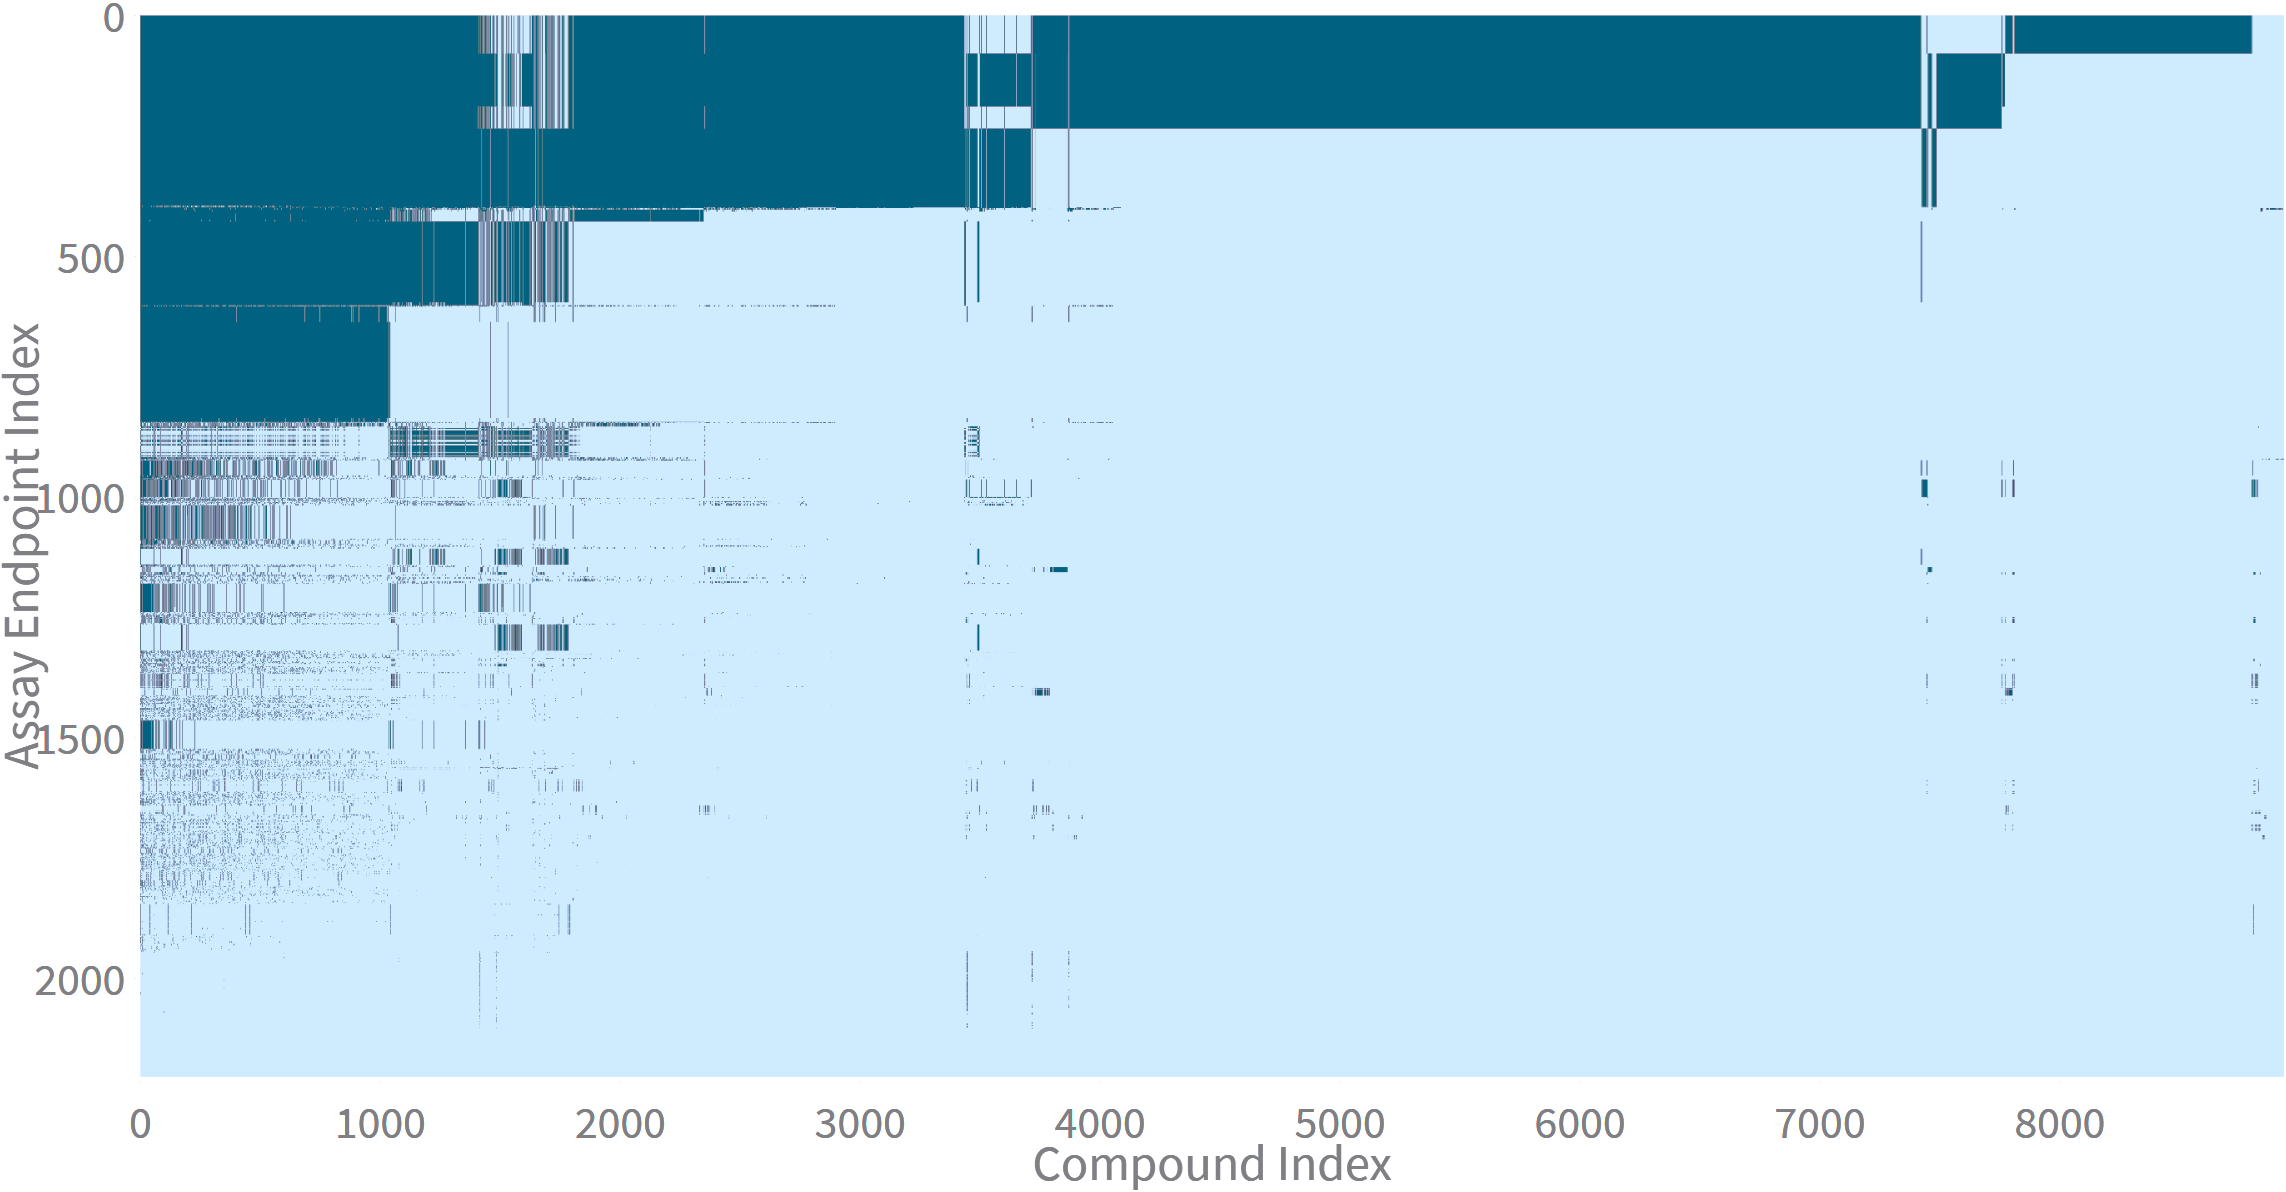
\includegraphics[width=1.0\textwidth]{figures/presence_matrix_all.png}  
    \caption{The \emph{presence matrix} $P$ covering all assay endpoints and compounds available in \textit{invitroDBv3.5} with $m = \num{2205}$ assay endpoints and $n = \num{9541}$ compounds. The count, where $P_{ij} = 1$, indicates the availability of \num{3342377} concentration-response series for downstream analysis.}
~\label{fig:presence_matrix_all} 
\end{figure}


A \textit{concentration-response series} is represented as a set of $k$ concentration-response pairs: 
\[ S = \{(conc_1, resp_1), (conc_2, resp_2), \dots, (conc_k, resp_k)\} \]
where $k$ $conc_i$ values are not necessarily unique. The quantity of concentration-response pairs exhibits considerable variability among different compounds tested across various assay endpoints.
In practice, concentrations are often subjected to multiple testing iterations, resulting in the formation of $n_{conc}$ distinct concentration groups. Within each concentration group, the number of replicates is indicated by $n_{rep}$.
Concentrations are transformed to the logarithmic scale using the unit $\mu M$ (micromolar), while the responses are normalized to either fold-induction or percent-of-control units.
Figure~\ref{fig:concentration_response_series} showcases a concentration-response series for a compound tested within a single assay endpoint.

\begin{figure}[htbp]  % Placement options: h (here), t (top), b (bottom), p (page)
    \centering
    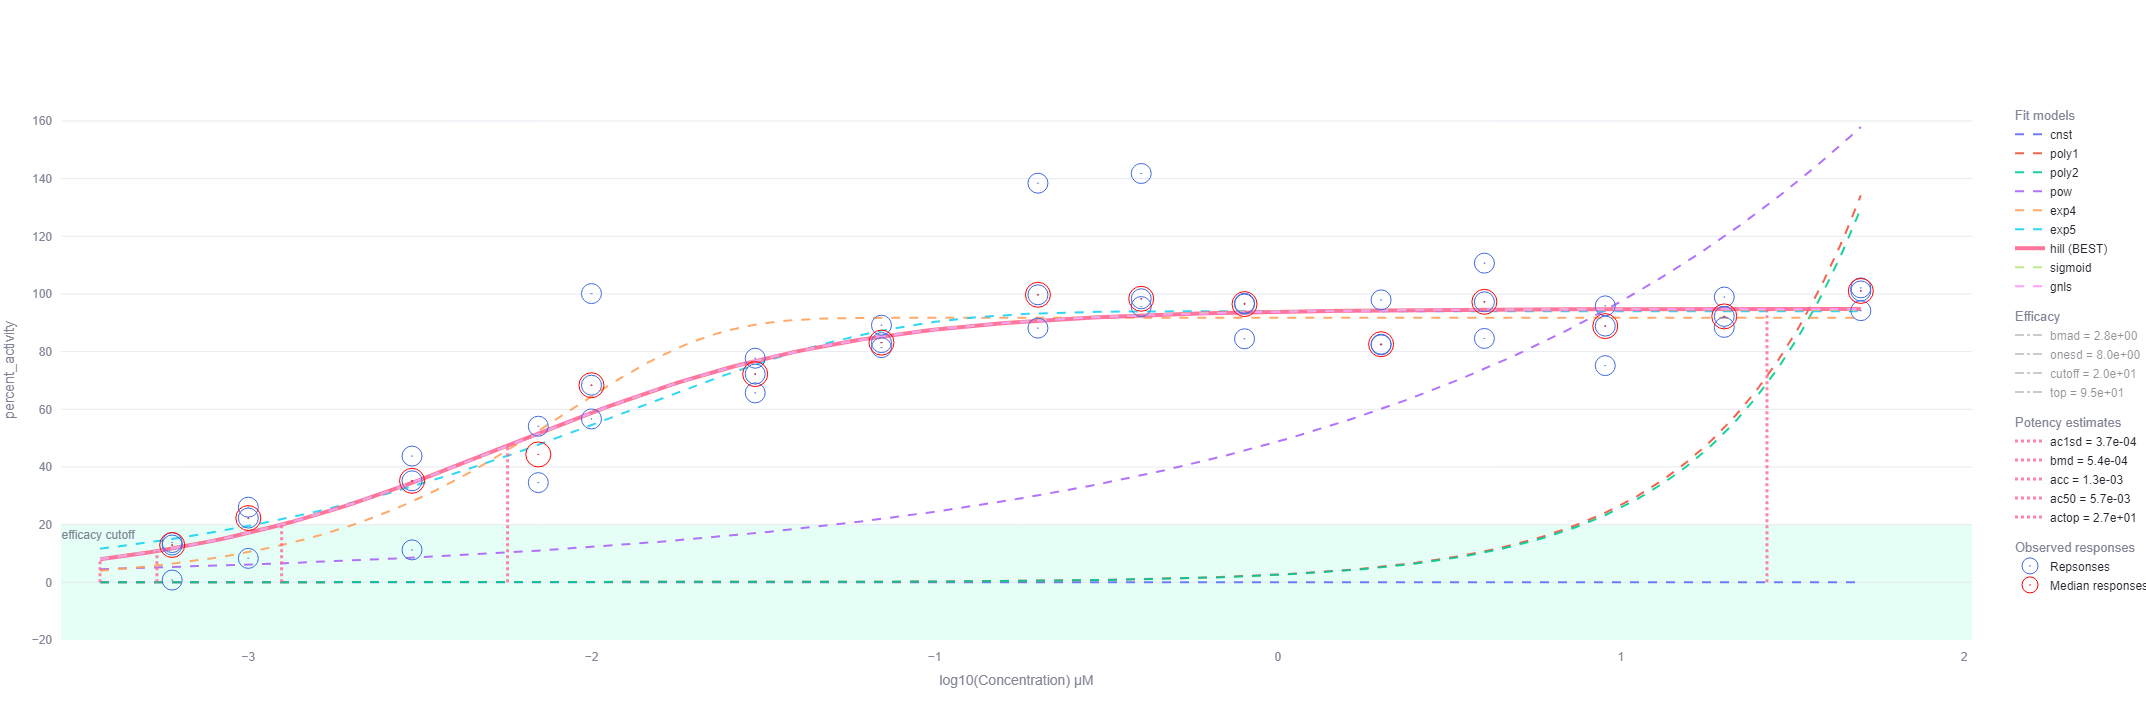
\includegraphics[width=1.0\textwidth]{figures/concentration_response_series_2.png}  
    \caption{A concentration-response series for the compound \textit{Estropipate} in the assay endpoint \textit{TOX21\_ERa\_LUC\_VM7\_Agonist}. The series has a total of $k = 45$ concentration-response pairs and is composed of $n_{conc} = 15$ concentration groups, each with $n_{rep} = 3$ replicates.}
~\label{fig:concentration_response_series} 
\end{figure}



\section{Pytcpl}
We introduce \href{https://github.com/rbBosshard/pytcpl}{pytcpl}, a streamlined Python package inspired by the R package \href{https://github.com/USEPA/CompTox-ToxCast-tcpl}{tcpl}, designed for processing high-throughput screening data. The package primarily focuses on providing essential features such as concentration-response curve fitting and allows for continuous hit-calling for compound bioactivity across diverse assay endpoints, akin to \href{https://github.com/USEPA/CompTox-ToxCast-tcplFit2}{tcplfit2}. \href{https://cfpub.epa.gov/si/si_public_record_Report.cfm?dirEntryId=355484&Lab=CCTE}{Invitrodb version 3.5 release} can optionally serve as backend database if desired. The package optimizes data storage and provides compressed raw data and metadata from \emph{invitroDB} in Parquet files. This efficient strategy reduces storage needs, resulting in just 4 GB within the repository—compared to the original 80 GB database. This obviates the need for a cumbersome, large-scale database installation, rendering downstream analysis more accessible and efficient. Our package is crafted to accomodate cusomizable processing steps and facilitate interactive data visualization with \href{https://pytcpl.streamlit.app/}{curve surfer} and empowers Python-oriented researchers to seamlessly engage in data analysis and exploration.
\subsection{Preprocessing}
First, all datapoints are collected from the database and assigned to the concentration response-series belonging to the respective ocompoud in the corresponding assay endpoint. The data is then filtered by the following criteria:

Data collection
Compute efficacy cutoff
Meet onditions for curve fitting
\subsection{Curve Fitting}
Introduce all candidate fit models
\subsection{Hit Calling}
Akaike criterion, 3 probabilities 
\subsection{Curve Surfer}
Data visualization, overview of what is possible with the tool. Filter by assay endpoint, compound, etc.


\section{Machine Learning Pipeline}
\subsection{Preprocessing}
Subselecting the columns from the output tables generated by pytcpl: DTXSID identifier and continuous hitcall value. The feature inputs to the machine learning model is a molecular structure represented as fingerprint generated from a SMILES string uniquely determined by the compounds DTXSID identifier. The SMILES string is a linear representation of a compound's molecular structure. The SMILES string is converted to a molecular graph, which is then converted to a feature vector. The feature vector is then used to train a machine learning model. The machine learning model is then used to predict the hitcall value for a given compound. The machine learning pipeline is illustrated in Figure~\ref{fig:ml_pipeline}. 


\subsection{Binary Classification}
The goal is to predict whether a compound is active or inactive for a given assay endpoint. We can formulate this as a binary classification problem, where the input is the compound's molecular structure fingerprint and the output is the hitcall value binarized by some decision threshold. The hitcall value is rendered to a binary variable, where 1 indicates that the compound is active and 0 indicates that the compound is inactive.
\subsection{Regression}
\subsection{Massbank Validation}

\chapter{Results and Discussion}\label{chap:results_discussion}
\section{Binary Classification}
\subsection{Metrics}
When assessing the performance of a binary prediction model using a validation dataset containing known target values, four key metrics come into play:

\begin{itemize}
  \item True Positives (TP): The number of correctly predicted active cases.
  \item True Negatives (TN): The number of correctly predicted inactive cases.
  \item False Positives (FP): The number of incorrectly predicted active cases.
  \item False Negatives (FN): The number of incorrectly predicted inactive cases.
\end{itemize}


Using these four values, it is possible to construct a confusion matrix, as illustrated in Table~\ref{tab:confusion_matrix}.

\begin{table}[h]
  \centering
  \caption{Confusion Matrix}
  \label{tab:confusion_matrix}
  \setlength{\tabcolsep}{10pt} % Adjust cell padding
  \renewcommand{\arraystretch}{1.5} % Adjust cell height
  \begin{tabular}{|c|c|c|}
  \cline{2-3}
  \multicolumn{1}{c|}{} & Actual Negative & Actual Positive \\
  \hline
  Predicted Negative & TN & FN \\
  \hline
  Predicted Positive & FP & TP \\
  \hline
  \end{tabular}
\end{table}

In binary classification, the classification threshold is a crucial parameter dictating how the model assigns data points to one of two classes based on predicted probabilities or scores. This threshold significantly influences the model's metrics, as illustrated in Figure~\ref{fig:classification_threshold}.
\begin{figure} 
  \centering
  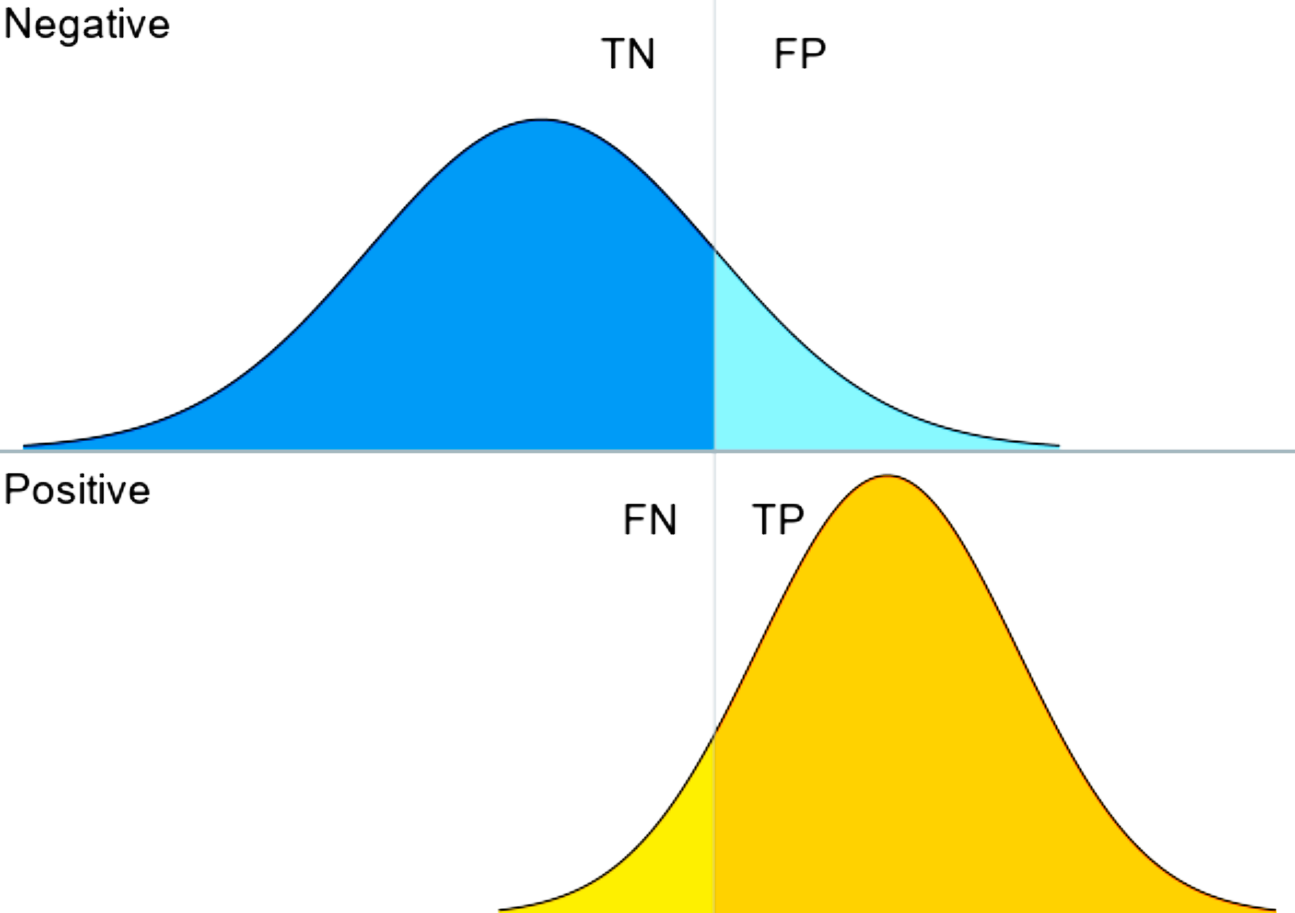
\includegraphics[width=0.5\textwidth]{figures/classification_threshold.png}
  \caption{Relationship between threshold and classification. Figure obtained from~\cite{wicklin2020}}
~\label{fig:classification_threshold}
\end{figure}

Several evaluation metrics can help assess the performance of a predictive model. These metrics include:

\begin{itemize}
  \item \textbf{Accuracy}: The ratio of correctly classified instances (TP) and (TN) to the total number of instances. It provides a general measure of the model's correctness.
  \[ \text{Accuracy}  A = \frac{TP + TN}{TP + TN + FP + FN} \]

  \item \textbf{Precision (P)}: The proportion of correctly predicted active cases (TP) to all instances predicted as active (TP + FP). 
  \[ \text{Precision } P = \frac{TP}{TP + FP} \]

  \item \textbf{Recall (R) or Sensitivity or True Positive Rate (TPR)}: The proportion of correctly predicted active cases (TP) to all actual active cases (TP + FN).
  \[ \text{Recall } R = \frac{TP}{TP + FN} \]

  \item \textbf{F1 Score}: The harmonic mean of precision and recall, which balances the trade-off between false positives and false negatives.
  \[ F1 = \frac{2 \cdot P \cdot R}{P + R} \]

  \item \textbf{True Negative Rate (TNR) Specificity}: The proportion of correctly predicted inactive cases (TN) to all actual inactive cases (TN + FP).
  \[ TNR = \frac{TN}{TN + FP} \]

  \item \textbf{Receiver Operating Characteristic (ROC) Curve}: A graphical representation of the model's performance across different classification thresholds. It plots the true positive rate (TNR) against the false positive rate (FPR).
  
\end{itemize}


\subsubsection{Imbalanced Data}
Exemplified in Figure~\ref{fig:confusion_matrix}, the majority of assay endpoints exhibit an imbalance in the distribution of active (positive) and inactive (negative) compounds when employing binarized toxicity hitcalls. Mostly the negative class significantly outweighs the postive class. Imbalanced datasets can lead to skewed performance metrics, as the model may perform well on the majority class but poorly on the minority class. To address imbalanced datasets, additional metrics such as macro-averaged and weighted-averaged metrics can be taken into account.
\begin{figure}[h]
  \centering
  \includegraphics[width=0.7\textwidth]{figures/roc97.png}
  \caption{For assay endpoint with aeid: 97, the Receiver Operating Characteristic (ROC) curve is shown for the XGBoost Classifier. We predicted each trained model with four different classification thresholds, namely default = 0.5, optimal = cost(TPR, FPR), True Positive Rate = 0.5 (tnr), True Negative Rate = 0.5 (tnr).}
~\label{fig:confusion_matrix}
\end{figure}


\begin{figure} 
  \centering
  \includegraphics[width=1.0\textwidth]{figures/cm97.png}
  \caption{For assay endpoint with aeid: 97, confusion matrices are shown for four different classification thresholds.}
~\label{fig:confusion_matrix}
\end{figure}

The majority of assay endpoints exhibit an imbalance in the distribution of active (positive) and inactive (negative) compounds when employing binarized toxicity hitcalls. Mostly the negative class significantly outweighs the postive class. Imbalanced datasets can lead to skewed performance metrics, as the model may perform well on the majority class but poorly on the minority class. To address imbalanced datasets, additional metrics such as macro-averaged and weighted-averaged metrics can be taken into account.

In macro-averaging, the metric is computed separately for each class, and then an unweighted average is taken. This approach assigns equal importance to each class, regardless of their representation within the dataset. As an example, macro-averaged precision calculates the unweighted average of precision across all classes, whereas the weighted-average of precision considers the impact of class prevalence.
\[ \text{Macro-Precision } = \frac{1}{N} \sum_{i=1}^{N} P_i \] 
\[ \text{Weighted-Precision } = \frac{1}{N} \sum_{i=1}^{N} \left(\frac{TP_i}{TP_i + FP_i}\right) \cdot \frac{N_i}{N} \]

In both cases, $N$ is the total number of classes (e.g. $N=2$ for the binary case), and $N_i$ represents the number of samples in class $i$. Similarly the macro-averaged and weighted-averaged recall and F1 score can be calculated.



\subsection{Performance}
We evaluated the model performance using the previously mentioned metrics. The following figures show the performance metrics applied to:

\begin{enumerate}
  \item the internal validation dataset (Figure~\ref{fig:hitcall_classification_xgb_val_default_macro_avg},~\ref{fig:hitcall_classification_xgb_val_default_weighted_avg},~\ref{fig:hitcall_classification_xgb_val_default_true},~\ref{fig:hitcall_classification_xgb_val_default_false})
  \item the fingerprint from the MassBank structure validation set (\ref{fig:hitcall_classification_xgb_val_default_macro_avg},~\ref{fig:hitcall_classification_xgb_val_default_weighted_avg},~\ref{fig:hitcall_classification_xgb_val_default_true},~\ref{fig:hitcall_classification_xgb_val_default_false})
  \item the SIRIUS-predicted fingerprint from the MassBank validation set (\ref{fig:hitcall_classification_xgb_val_default_macro_avg},~\ref{fig:hitcall_classification_xgb_val_default_weighted_avg},~\ref{fig:hitcall_classification_xgb_val_default_true},~\ref{fig:hitcall_classification_xgb_val_default_false})
\end{enumerate}

For each validation set, four figures are presented, each of which shows a different perspective on the performance metrics:

\begin{enumerate}
  \item the \emph{macro average} metrics
  \item the \emph{weighted average} metrics
  \item the separately sliced metrics for the \emph{positive} class
  \item the separately sliced metrics for the \emph{negative} class
\end{enumerate}

The default classification threshold, which is 0.5, was used for predicting the class labels. Each figure shows performance on the binarized hitcall without cytotoxicity correction, in a scatter plot that compares precision against recall for all target assay endpoints employing each of the classifiers. All models use an XGBoost classifier as the underlying feature selection model. The marker size in the scatter plots reflects the varying number of compounds in the validation set across the assay endpoints. The marginal boxplots illustrate the distribution of the performance metrics across the target assay endpoint models. The adjacent table provides the average metrics for the estimators across all target assay endpoint models.


\subsubsection{Internal validation}
\begin{figure}[h]
  \centering
  \includegraphics[width=0.99\textwidth]{figures/hitcall_classification_xgb_val_default_macro_avg.png}
  \caption{}
~\label{fig:hitcall_classification_xgb_val_default_macro_avg}
\end{figure}

\begin{figure}[h]
  \centering
  \includegraphics[width=0.99\textwidth]{figures/hitcall_classification_xgb_val_default_weighted_avg.png}
  \caption{}
~\label{fig:hitcall_classification_xgb_val_default_weighted_avg}
\end{figure}

\begin{figure}[h]
  \centering
  \includegraphics[width=0.99\textwidth]{figures/hitcall_classification_xgb_val_default_true.png}
  \caption{}
~\label{fig:hitcall_classification_xgb_val_default_true}
\end{figure}

\begin{figure}[h]
  \centering
  \includegraphics[width=0.99\textwidth]{figures/hitcall_classification_xgb_val_default_false.png}
  \caption{}
~\label{fig:hitcall_classification_xgb_val_default_false}
\end{figure}

\subsubsection{MassBank structure validation}
\begin{figure}[h]
  \centering
  \includegraphics[width=0.99\textwidth]{figures/hitcall_classification_xgb_val_default_macro_avg.png}
  \caption{}
  ~\label{fig:hitcall_classification_xgb_val_default_false}
\end{figure}


Perfromance results were generated for every combination of the three validation sets, the two target variables (hitcall, cytotoxicity corrected hitcall),  $\geq 300$ assay endpoints, two feature selection models (XGBoost, RandomForest), four classiifaction thresholds (default, optimal, TPR=0.5, TNR=0.5). 
\chapter{Conclusion}


In summary, the performance results were explored across diverse combinations of metrics and models, providing a thorough understanding of the model's capabilities in various scenarios. This analysis allowed for a deeper comprehension of the strengths and weaknesses of the binary classification models employed in hazard assessment.
% \chapter{Writing scientific texts in English}

This chapter was originally a separate document written by Reto
Spöhel.  It is reprinted here so that the template can serve as a
quick guide to thesis writing, and to provide some more example
material to give you a feeling for good typesetting.

% We're going to need an extra theorem-like environment for this
% chapter
\theoremstyle{plain}
\theoremsymbol{}
\newtheorem{Rule}[theorem]{Rule}

\section{Basic writing rules}

The following rules need little further explanation; they are best
understood by looking at the example in the booklet by Knuth et al.,
§2--§3.

\begin{Rule}
  Write texts, not chains of formulas.
\end{Rule}

More specifically, write full sentences that are logically
interconnected by phrases like `Therefore', `However', `On the other
hand', etc.\ where appropriate.

\begin{Rule}
  Displayed formulas should be embedded in your text and punctuated
  with it.
\end{Rule}

In other words, your writing should not be divided into `text parts'
and `formula parts'; instead the formulas should be tied together by
your prose such that there is a natural flow to your writing.

\section{Being nice to the reader}

Try to write your text in such a way that a reader enjoys reading
it. That's of course a lofty goal, but nevertheless one you should
aspire to!

\begin{Rule}
  Be nice to the reader.
\end{Rule}

Give some intuition or easy example for definitions and theorems which
might be hard to digest. Remind the reader of notations you introduced
many pages ago -- chances are he has forgotten them. Illustrate your
writing with diagrams and pictures where this helps the reader. Etc.

\begin{Rule}
  Organize your writing.
\end{Rule}

Think carefully about how you subdivide your thesis into chapters,
sections, and possibly subsections.  Give overviews at the beginning
of your thesis and of each chapter, so the reader knows what to
expect. In proofs, outline the main ideas before going into technical
details. Give the reader the opportunity to `catch up with you' by
summing up your findings periodically.

\emph{Useful phrases:} `So far we have shown that \ldots', `It remains
to show that \ldots', `Recall that we want to prove inequality (7), as
this will allow us to deduce that \ldots', `Thus we can conclude that
\ldots. Next, we would like to find out whether \ldots', etc.

\begin{Rule}
  Don't say the same thing twice without telling the reader that you
  are saying it twice.
\end{Rule}

Repetition of key ideas is important and helpful. However, if you
present the same idea, definition or observation twice (in the same or
different words) without telling the reader, he will be looking for
something new where there is nothing new.

\emph{Useful phrases:} `Recall that [we have seen in Chapter 5 that]
\ldots', `As argued before / in the proof of Lemma 3, \ldots', `As
mentioned in the introduction, \ldots', `In other words, \ldots', etc.

\begin{Rule}
  Don't make statements that you will justify later without telling
  the reader that you will justify them later.
\end{Rule}

This rule also applies when the justification is coming right in the
next sentence!  The reasoning should be clear: if you violate it, the
reader will lose valuable time trying to figure out on his own what
you were going to explain to him anyway.

\emph{Useful phrases:} `Next we argue that \ldots', `As we shall see,
\ldots', `We will see in the next section that \ldots, etc.


\section{A few important grammar rules}

\begin{Rule}
  \label{rule:no-comma-before-that}
  There is (almost) \emph{never} a comma before `that'.
\end{Rule}

It's really that simple. Examples:
\begin{quote}
  We assume that \ldots\\
  \emph{Wir nehmen an, dass \ldots}

  It follows that \ldots\\
  \emph{Daraus folgt, dass \ldots}

  `thrice' is a word that is seldom used.\\
  \emph{`thrice' ist ein Wort, das selten verwendet wird.}
\end{quote}
Exceptions to this rule are rare and usually pretty obvious. For
example, you may end up with a comma before `that' because `i.e.' is
spelled out as `that is':
\begin{quote}
  For \(p(n)=\log n/n\) we have \ldots{} However, if we choose \(p\) a
  little bit higher, that is \(p(n)=(1+\varepsilon)\log n/n\) for some
  \(\varepsilon>0\), we obtain that\ldots
\end{quote}
Or you may get a comma before `that' because there is some additional
information inserted in the middle of your sentence:
\begin{quote}
  Thus we found a number, namely \(n_0\), that satisfies equation (13).
\end{quote}
If the additional information is left out, the sentence has no comma:
\begin{quote}
  Thus we found a number that satisfies equation (13).
\end{quote}
(For `that' as a relative pronoun, see also
Rules~\ref{rule:non-defining-has-comma}
and~\ref{rule:defining-without-comma} below.)

\begin{Rule}
  There is usually no comma before `if'.
\end{Rule}

Example:
\begin{quote}
  A graph is not \(3\)-colorable if it contains a \(4\)-clique.\\
  \emph{Ein Graph ist nicht \(3\)-färbbar, wenn er eine \(4\)-Clique
    enthält.}
\end{quote}
However, if the `if' clause comes first, it is usually separated from
the main clause by a comma:
\begin{quote}
  If a graph contains a \(4\)-clique, it is not \(3\)-colorable .\\
  \emph{Wenn ein Graph eine \(4\)-Clique enthält, ist er nicht
    \(3\)-färbbar.}
\end{quote}

There are more exceptions to these rules than to
Rule~\ref{rule:no-comma-before-that}, which is why we are not
discussing them here. Just keep in mind: don't put a comma before `if'
without good reason.

\begin{Rule}
  \label{rule:non-defining-has-comma}
  Non-defining relative clauses have commas.
\end{Rule}
\begin{Rule}
  \label{rule:defining-without-comma}
  Defining relative clauses have no commas.
\end{Rule}

In English, it is very important to distinguish between two types of
relative clauses: defining and non-defining ones. This is a
distinction you absolutely need to understand to write scientific
texts, because mistakes in this area actually distort the meaning of
your text!

It's probably easier to explain first what a \emph{non-defining}
relative clause is. A non-defining relative clauses simply gives
additional information \emph{that could also be left out} (or given in
a separate sentence). For example, the sentence
\begin{quote}
  The \textsc{WeirdSort} algorithm, which was found by the famous
  mathematician John Doe, is theoretically best possible but difficult
  to implement in practice.
\end{quote}
would be fully understandable if the relative clause were left out
completely. It could also be rephrased as two separate sentences:
\begin{quote}
  The \textsc{WeirdSort} algorithm is theoretically best possible but
  difficult to implement in practice. [By the way,] \textsc{WeirdSort}
  was found by the famous mathematician John Doe.
\end{quote}
This is what a non-defining relative clause is. \emph{Non-defining
  relative clauses are always written with commas.} As a corollary we
obtain that you cannot use `that' in non-defining relative clauses
(see Rule~\ref{rule:no-comma-before-that}!). It would be wrong to
write
\begin{quote}
  \st{The \textsc{WeirdSort} algorithm, that was found by the famous
    mathematician John Doe, is theoretically best possible but
    difficult to implement in practice.}
\end{quote}
A special case that warrants its own example is when `which' is
referring to the entire preceding sentence:
\begin{quote}
  Thus inequality (7) is true, which implies that the Riemann
  hypothesis holds.
\end{quote}
As before, this is a non-defining relative sentence (it could be left
out) and therefore needs a comma.

So let's discuss \emph{defining} relative clauses next. A defining
relative clause tells the reader \emph{which specific item the main
  clause is talking about}. Leaving it out either changes the meaning
of the sentence or renders it incomprehensible altogether.  Consider
the following example:

\begin{quote}
  The \textsc{WeirdSort} algorithm is difficult to implement in
  practice. In contrast, the algorithm that we suggest is very simple.
\end{quote}

Here the relative clause `that we suggest' cannot be left out -- the
remaining sentence would make no sense since the reader would not know
which algorithm it is talking about. This is what a defining relative
clause is. \textit{Defining relative clauses are never written with
  commas.} Usually, you can use both `that' and `which' in defining
relative clauses, although in many cases `that' sounds better.

As a final example, consider the following sentence:
\begin{quote}
  For the elements in \(\mathcal{B}\) which satisfy property (A), we
  know that equation (37) holds.
\end{quote}
This sentence does not make a statement about all elements in
\(\mathcal{B}\), only about those satisfying property (A). The relative
clause is \emph{defining}. (Thus we could also use `that' in place of
`which'.)

In contrast, if we add a comma the sentence reads
\begin{quote}
  For the elements in \(\mathcal{B}\), which satisfy property (A), we
  know that equation (37) holds.
\end{quote}

Now the relative clause is \emph{non-defining} -- it just mentions in
passing that all elements in \(\mathcal{B}\) satisfy property (A). The
main clause states that equation (37) holds for \emph{all} elements in
\(\mathcal{B}\). See the difference?


\section[Things you (usually) don't say in English]%
{Things you (usually) don't say in English -- and what to say
  instead}
\label{sec:list}

Table~\ref{tab:things-you-dont-say} lists some common mistakes and
alternatives.  The entries should not be taken as gospel -- they don't
necessarily mean that a given word or formulation is wrong under all
circumstances (obviously, this depends a lot on the context). However,
in nine out of ten instances the suggested alternative is the better
word to use.

\begin{table}
  \centering
  \caption{Things you (usually) don't say}
  \label{tab:things-you-dont-say}
  \begin{tabular}{lll}
    \toprule
    \st{It holds (that) \dots} & We have \dots & \emph{Es gilt \dots}\\
    \multicolumn{3}{l}{\quad\footnotesize(`Equation (5) holds.' is fine, though.)}\\
    \st{$x$ fulfills property $\mathcal{P}$.}& \(x\) satisfies property \(\mathcal{P}\). & \emph{\(x\) erfüllt Eigenschaft \(\mathcal{P}\).} \\
    \st{in average} & on average & \emph{im Durchschnitt}\\
    \st{estimation} & estimate   & \emph{Abschätzung}\\
    \st{composed number} & composite number & \emph{zusammengesetzte Zahl}\\
    \st{with the help of} & using & \emph{mit Hilfe von}\\
    \st{surely} & clearly & \emph{sicher, bestimmt}\\
    \st{monotonously increasing} & monotonically incr. & \emph{monoton steigend}\\
    \multicolumn{3}{l}{\quad\footnotesize(Actually, in most cases `increasing' is just fine.)}\\
    \bottomrule
  \end{tabular}
\end{table}

%%% Local Variables:
%%% mode: latex
%%% TeX-master: "thesis"
%%% End:

% \chapter{Typography}


\section{Punctuation}

\begin{Rule}
  Use opening (`) and closing (') quotation marks correctly.
\end{Rule}

In \LaTeX, the closing quotation mark is typed like a normal
apostrophe, while the opening quotation mark is typed using the French
\emph{accent grave} on your keyboard (the \emph{accent grave} is the
one going down, as in \emph{frère}).

Note that any punctuation that \emph{semantically} follows quoted
speech goes inside the quotes in American English, but outside in
Britain.  Also, Americans use double quotes first.  Oppose
\begin{quote}
  ``Using `lasers,' we punch a hole in \ldots\ the Ozone Layer,''
  Dr.\ Evil said.
\end{quote}
to
\begin{quote}
  `Using ``lasers'', we punch a hole in \ldots\ the Ozone Layer',
  Dr.\ Evil said.
\end{quote}

\begin{Rule}
  Use hyphens (-), en-dashes (--) and em-dashes (---) correctly.
\end{Rule}

A hyphen is only used in words like `well-known', `$3$-colorable'
etc., or to separate words that continue in the next line (which is
known as hyphenation).  It is entered as a single ASCII hyphen
character (\texttt{-}).

To denote ranges of numbers, chapters, etc., use an en-dash (entered
as two ASCII hyphens \texttt{--}) with no spaces on either side.  For
example, using Equations (1)--(3), we see\ldots

As the equivalent of the German \emph{Gedankenstrich}, use an en-dash
with spaces on both sides -- in the title of Section \ref{sec:list},
it would be wrong to use a hyphen instead of the dash. (Some English
authors use the even longer emdash (---) instead, which is typed as
three subsequent hyphens in \LaTeX. This emdash is used without spaces
around it---like so.)


\section{Spacing}

\begin{Rule}
  \label{rule:no-manual-spacing}
  Do not add spacing manually.
\end{Rule}

You should never use the commands \lstinline-\\- (except within
tabulars and arrays), \lstinline[showspaces=true]-\ - (except to
prevent a sentence-ending space after Dr.\ and such),
\lstinline-\vspace-, \lstinline-\hspace-, etc.  The choices programmed
into \LaTeX{} and this style should cover almost all cases.  Doing it
manually quickly leads to inconsistent spacing, which looks terrible.
Note that this list of commands is by no means conclusive.

\begin{Rule}
  Judiciously insert spacing in maths where it helps.
\end{Rule}

This directly contradicts Rule~\ref{rule:no-manual-spacing}, but in
some cases \TeX{} fails to correctly decide how much spacing is
required.  For example, consider
\begin{displaymath}
  f(a,b) = f(a+b, a-b).
\end{displaymath}
In such cases, inserting a thin math space \lstinline-\,- greatly
increases readability:
\begin{displaymath}
  f(a,b) = f(a+b,\, a-b).
\end{displaymath}

Along similar lines, there are variations of some symbols with
different spacing.  For example, Lagrange's Theorem states that
\(\abs{G}=[G:H]\abs{H}\), but the proof uses a bijection \(f\colon
aH\to bH\).  (Note how the first colon is symmetrically spaced, but
the second is not.)

\begin{Rule}
  Learn when to use \lstinline[showspaces=true]-\ - and
  \lstinline-\@-.
\end{Rule}

Unless you use `french spacing', the space at the end of a sentence is
slightly larger than the normal interword space.

The rule used by \TeX{} is that any space following a period,
exclamation mark or question mark is sentence-ending, except for
periods preceded by an upper-case letter.  Inserting \lstinline-\-
before a space turns it into an interword space, and inserting
\lstinline-\@- before a period makes it sentence-ending.  This means
you should write
\begin{lstlisting}
Prof.\ Dr.\ A. Steger is a member of CADMO\@.
If you want to write a thesis with her, you
should use this template.
\end{lstlisting}
which turns into
\begin{quote}
  Prof.\ Dr.\ A. Steger is a member of CADMO\@.  If you want to write
  a thesis with her, you should use this template.
\end{quote}
The effect becomes more dramatic in lines that are stretched slightly
during justification:
\begin{quote}
  \parbox{\linewidth}{\hbox to \linewidth{%
      Prof.\ Dr.\ A. Steger is a member of CADMO\@.  If you}}
\end{quote}

\begin{Rule}
  Place a non-breaking space (\lstinline-~-) right before references.
\end{Rule}

This is actually a slight simplification of the real rule, which
should invoke common sense.  Place non-breaking spaces where a line
break would look `funny' because it occurs right in the middle of a
construction, especially between a reference type (Chapter) and its
number.


\section{Choice of `fonts'}

Professional typography distinguishes many font attributes, such as
family, size, shape, and weight.  The choice for sectional divisions
and layout elements has been made, but you will still occasionally
want to switch to something else to get the reader's attention.  The
most important rule is very simple.

\begin{Rule}
  When emphasising a short bit of text, use \lstinline-\emph-.
\end{Rule}

In particular, \emph{never} use bold text (\lstinline-\textbf-).
Italics (or Roman type if used within italics) avoids distracting the
eye with the huge blobs of ink in the middle of the text that bold
text so quickly introduces.

Occasionally you will need more notation, for example, a consistent
typeface used to identify algorithms.

\begin{Rule}
  Vary one attribute at a time.
\end{Rule}

For example, for \textsc{WeirdSort} we only changed the shape to small
caps.  Changing two attributes, say, to bold small caps would be
excessive (\LaTeX{} does not even have this particular variation).
The same holds for mathematical notation: the reader can easily
distinguish \(g_n\), \(G(x)\), \(\mathcal{G}\) and \(\mathsf{G}\).

\begin{Rule}
  Never underline or uppercase.
\end{Rule}

No exceptions to this one, unless you are writing your thesis on a
typewriter.  Manually.  Uphill both ways.  In a blizzard.


\section{Displayed equations}

\begin{Rule}
  Insert paragraph breaks \emph{after} displays only where they
  belong.  Never insert paragraph breaks \emph{before} displays.
\end{Rule}

\LaTeX{} translates sequences of more than one linebreak (i.e., what
looks like an empty line in the source code) into a paragraph break in
almost all contexts.  This also happens before and after displays,
where extra spacing is inserted to give a visual indication of the
structure.  Adding a blank line in these places may look nice in the
sources, but compare the resulting display

\begin{displaymath}
  a = b
\end{displaymath}

to the following:
\begin{displaymath}
  a = b
\end{displaymath}
The first display is surrounded by blank lines, but the second is not.
It is bad style to start a paragraph with a display (you should always
tell the reader what the display means first), so the rule follows.

\begin{Rule}
  Never use \lstinline-eqnarray-.
\end{Rule}

It is at the root of most ill-spaced multiline displays.  The
\package{amsmath} package provides better alternatives, such as the
\lstinline-align- family
\begin{align*}
  f(x) &= \sin x, \\
  g(x) &= \cos x,
\end{align*}
and \lstinline-multline- which copes with excessively long equations:
\begin{multline*}
  \def\P{\mathrm P}
  \P\bigl[X_{t_0} \in (z_0, z_0+dz_0],\ldots, X_{t_n}\in(z_n,z_n+dz_n]\bigr]
  \\= \nu(dz_0) K_{t_1}(z_0,dz_1) K_{t_2-t_1}(z_1,dz_2)\cdots
  K_{t_n-t_{n-1}}(z_{n-1},dz_n).
\end{multline*}


\section{Floats}

By default this style provides floating environments for tables and
figures.  The general structure should be as follows:
\begin{lstlisting}
\begin{figure}
  \centering
  % content goes here
  \caption{A short caption}
  \label{some-short-label}
\end{figure}
\end{lstlisting}
Note that the label must follow the caption, otherwise the label will
refer to the surrounding section instead.  Also note that figures
should be captioned at the bottom, and tables at the top.

The whole point of floats is that they, well, \emph{float} to a place
where they fit without interrupting the text body.  This is a frequent
source of confusion and changes; please leave it as is.

\begin{Rule}
  Do not restrict float movement to only `here'
  \textnormal{(\lstinline-h-)}.
\end{Rule}

If you are still tempted, you should avoid the float altogether and
just show the figure or table inline, similar to a displayed equation.

%%% Local Variables:
%%% mode: latex
%%% TeX-master: "thesis"
%%% End:

% \chapter{Example Chapter}

Dummy text.

\section{Example Section}

Dummy text.

\subsection{Example Subsection}

Dummy text.

\subsubsection{Example Subsubsection}

Dummy text.

\paragraph{Example Paragraph}

Dummy text.

\subparagraph{Example Subparagraph}

Dummy text.


% \backmatter  % Template v2 fixes: this just breaks things

% Template v2 fixes: Bibliography belongs before appendix
\printbibliography

\appendix
\chapter{Appendix}





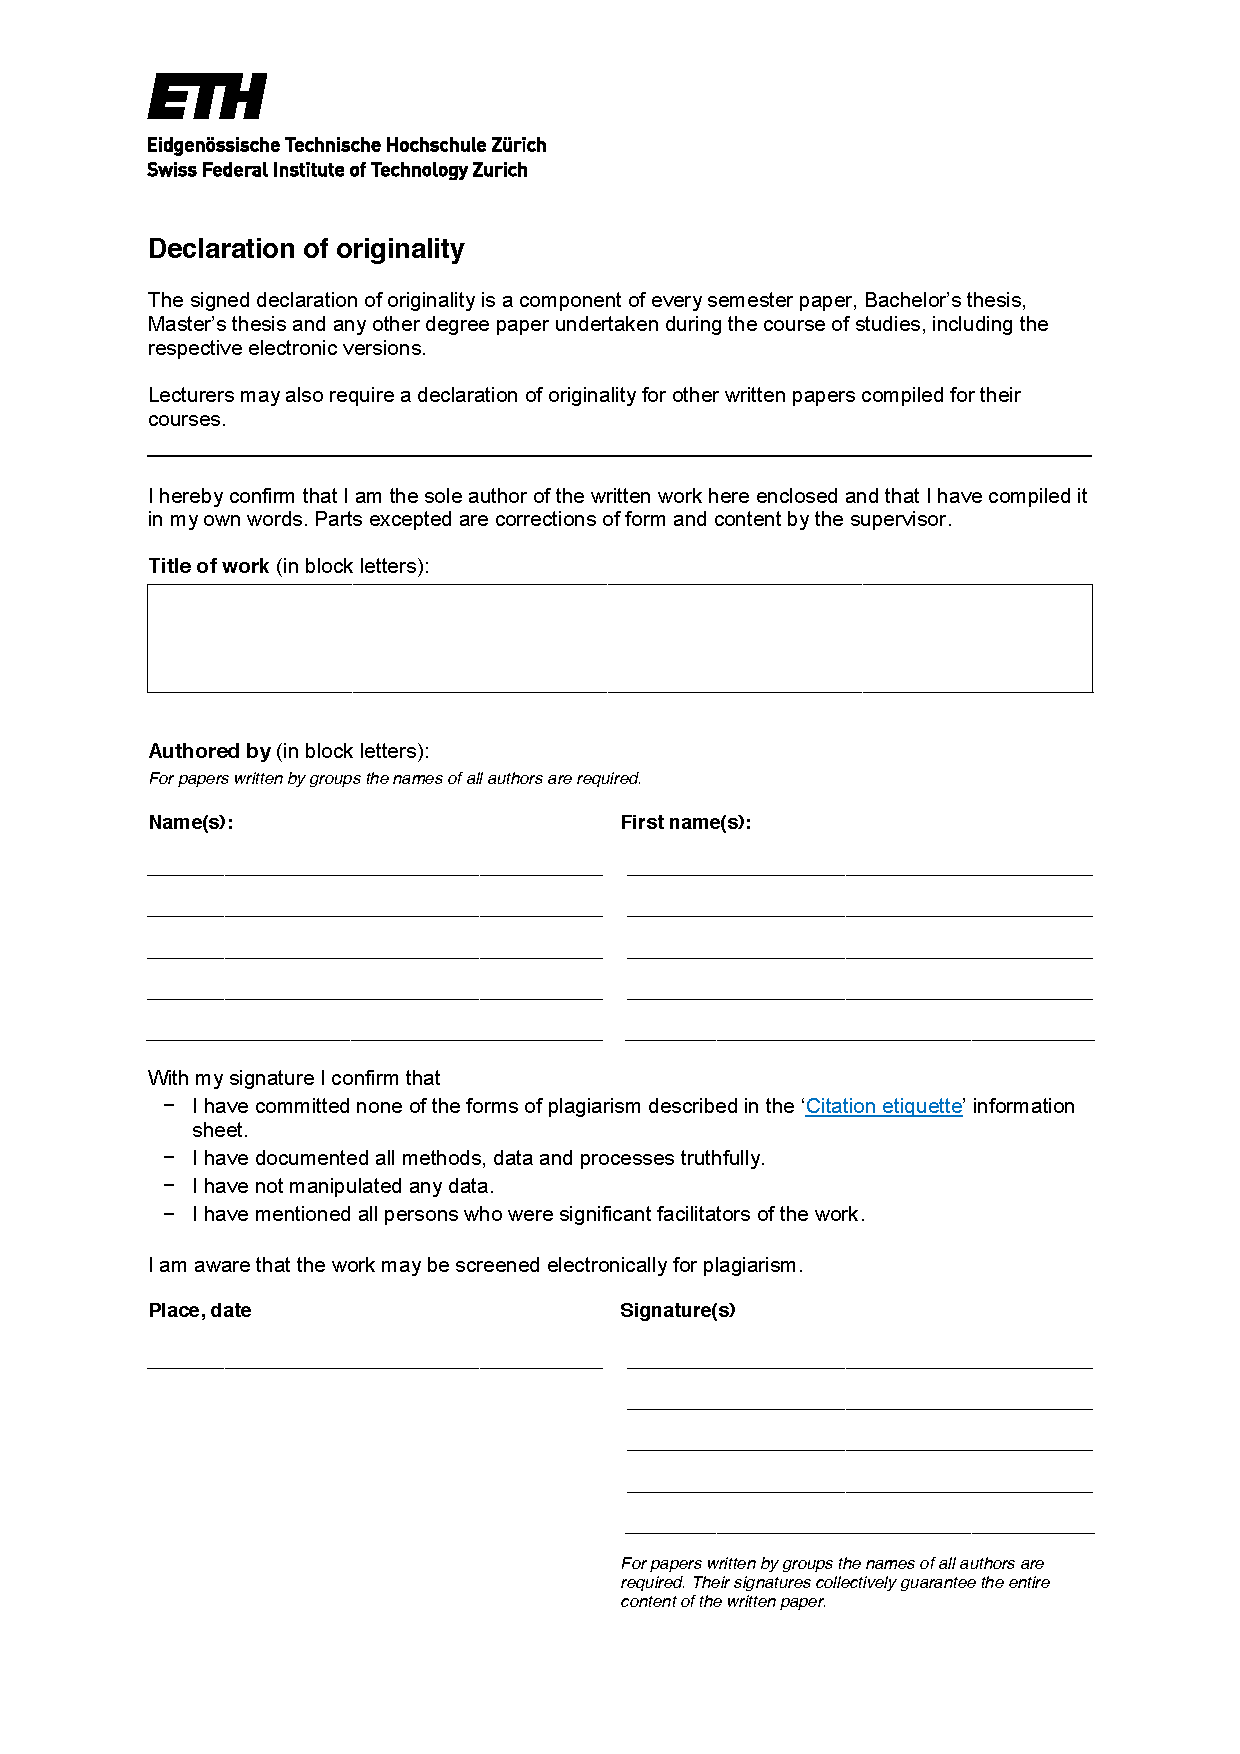
\includepdf[pages={-}]{eth-template/declaration-originality.pdf}

\end{document}
